\documentclass{article}
\usepackage{graphicx}
\usepackage{stix2}

\title{Introduction To Compiler Assignment 1 : Building GCC}
\author{201704150 Kangjun Heo}
\date{\today}

\begin{document}

\maketitle

\section{Introduction}
GCC is a source code compilation toolchain that is created and maintained by Free Software Foundation. 
It targets mainly C or C++, even Fortran and Go, Haskell. In this report, I will build GCC from source code
that is being distributed by official GNU repository.

Since GCC is a gigantic collection of software, we need to check prerequisites to build GCC successfully.
its details can be found at https://gcc.gnu.org/install/, this report follows this instructions as possible. 

\section{Preparation}

\subsection{Preparing toolchain}

\par GCC itself is written in ISO C++, especially conforms C++ 11 Standard. A compiler that supports modern C++
is required, I've prepared GCC 9.3.0 on WSL(Win- dows Subsystems for Linux) Ubuntu 20.04. It can be easily 
installed via \texttt{apt}, a good package manager for debian variant Linux distributions. \\

\begin{figure}[!htbp]
    \centering
    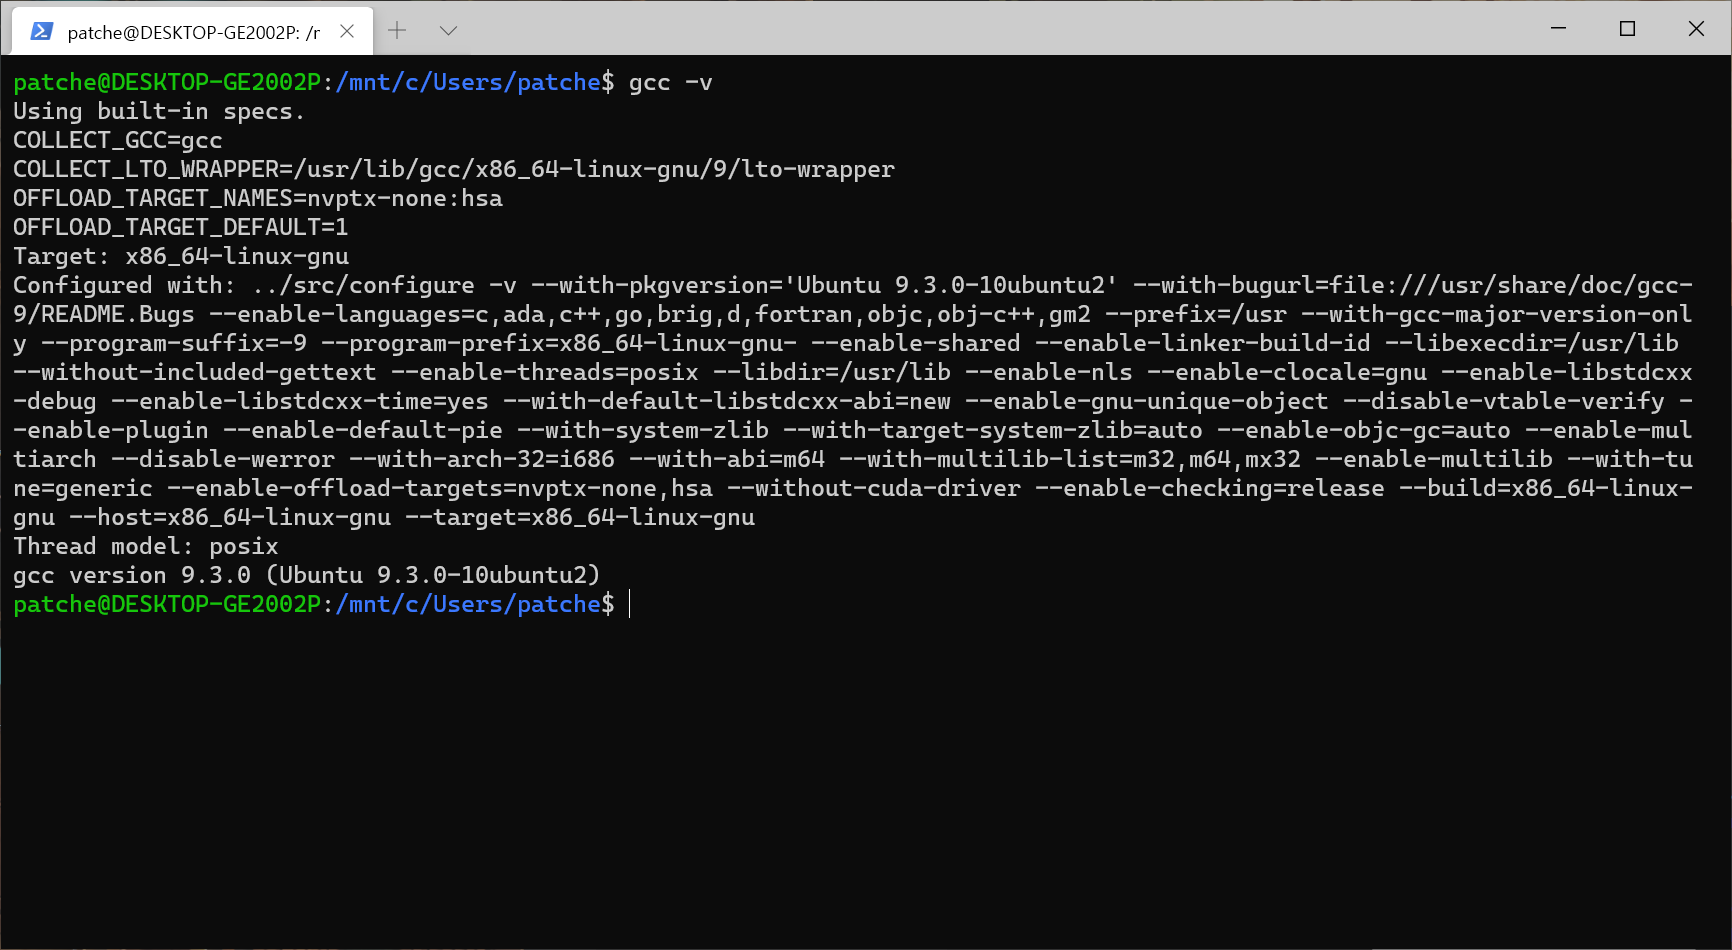
\includegraphics[width=0.8\textwidth]{images/1.png}
    \caption{GCC 9.3.0 with WSL Ubuntu}
\end{figure}

\par To install GCC in Ubuntu, execute following command: \\

\par \texttt{\# apt install gcc} \\

\par This will prepare appropriate set of gcc compilation infrastructure for you. \\


GNU Make is a tool for controlling software compilation and building. GCC uses \texttt{Makefile},
a script that is read and executed by Make. \\

\par To install Make, execute following command: \\

\par \texttt{\# apt install make} \\

And last, we need \texttt{git}, a version control system that is created by Linux Torvalds, well known
as father of Linux. Like Linux, GCC is also maintained with this system, so we need to install \texttt{git}
to retrieve its source code.\\

\par To install Make, execute following command: \\

\par \texttt{\# apt install git} \\

\subsection{Libraries}
GCC uses \texttt{GMP}, \texttt{MPFR}, \texttt{MPC}. These libraries are required not only 
for building GCC, but also for several optimizations of GCC functionalities. When these are contained as 
subdirectories in GCC sources, these will be built during build process.

\begin{itemize}
    \item GMP is required 4.3.2 or later.
    \item MPFR is required 3.1.0 or later.
    \item MPC is required 1.0.1 or later.
\end{itemize}

\subsection{Source code}
Of course, A valid set of GCC source code is required to build GCC. It is very popular
toolchain among developers around the world, we can find it with a lot of way. In this
report, I will use official GNU's git source tree. its url is: \\

\texttt{git://gcc.gnu.org/git/gcc.git}\\

To retrieve it, execute this command:\\

\texttt{\# git clone git://gcc.gnu.org/git/gcc.git}\\

\begin{figure}[!htbp]
    \centering
    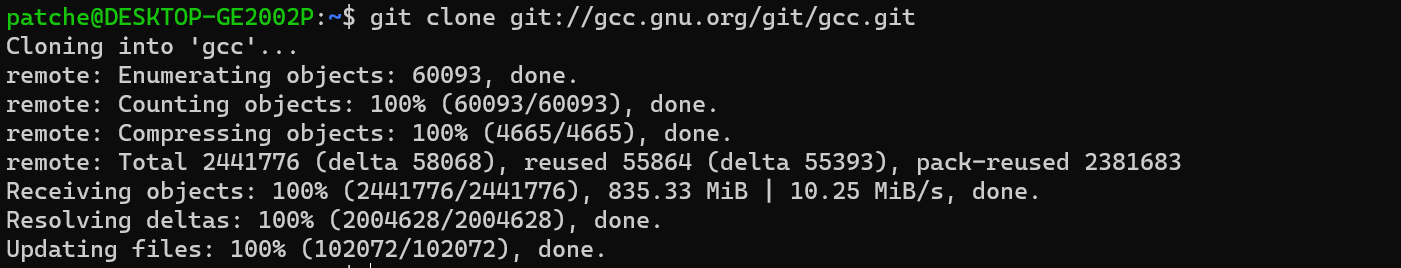
\includegraphics[width=0.9\textwidth]{images/2.png}
    \caption{Cloning GCC repository from official Git}
\end{figure}

\begin{figure}[!htbp]
    \centering
    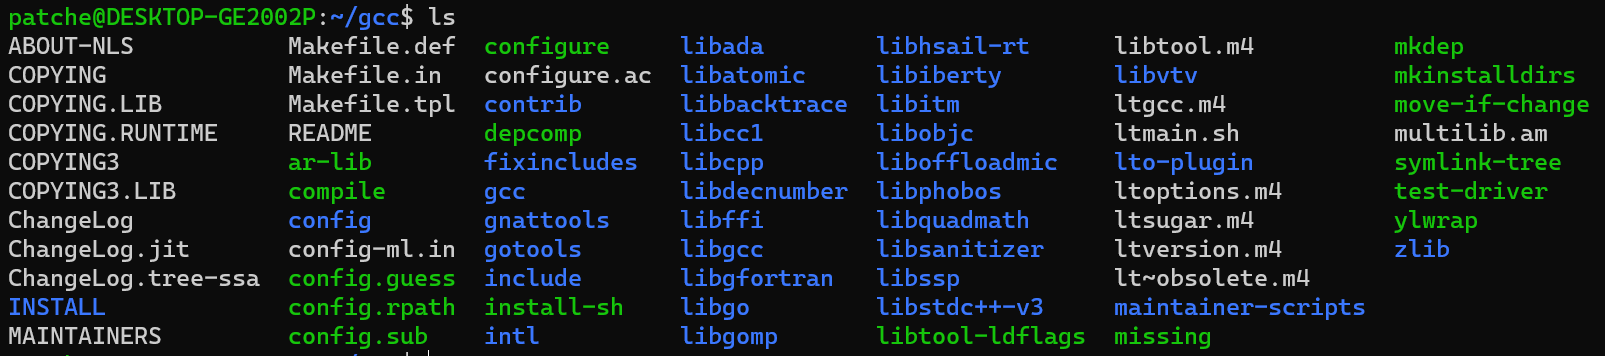
\includegraphics[width=0.9\textwidth]{images/3.png}
    \caption{Directory structues of cloned GCC source code}
\end{figure}

As I mentioned in \textbf{Libraries} subsection, these 3 directories should be created
for easy compilation of GCC. GCC provides a script to retrieve prerequisites in simple way,
just run \texttt{./contrib/download\_prerequisites}.

\begin{figure}[!htbp]
    \centering
    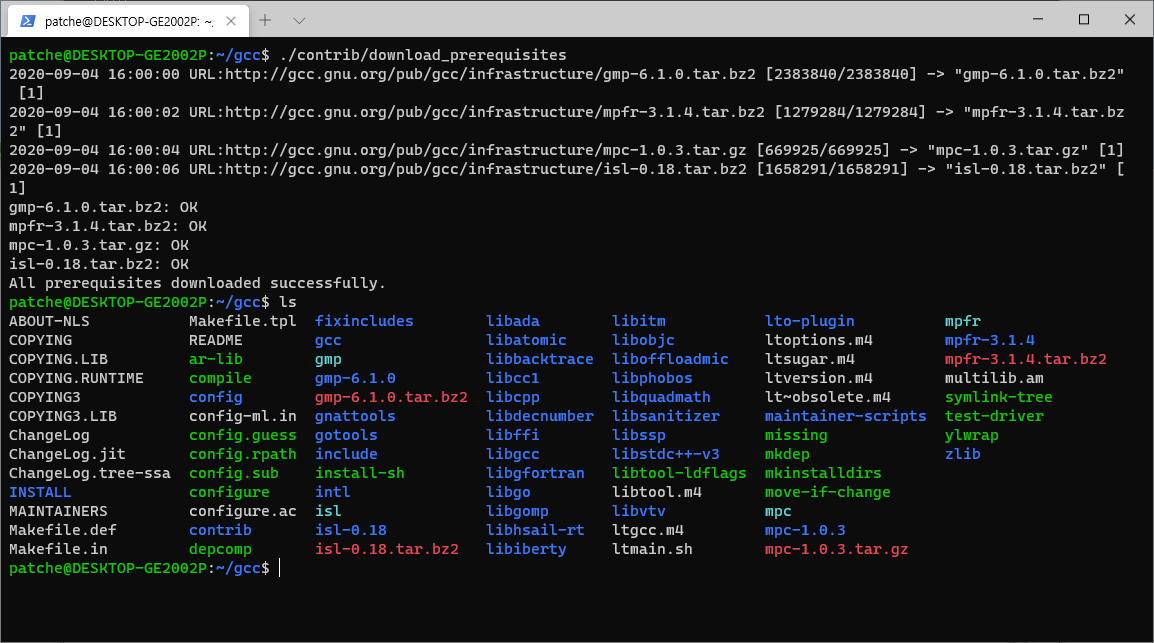
\includegraphics[width=0.8\textwidth]{images/5.png}
    \caption{GCC directory structure with prerequisites}
\end{figure}

\section{Building and Installation}
\subsection{Configuration}
GCC supports various kind of machines, and languages. Prior to compile and build GCC, 
we need to configure its specification. \texttt{configure} script helps this process,
its manual is located at https://gcc.gnu.org/install/configure.html. I am not going to
use built GCC for other architectures, also target C and C++ only, \texttt{configure}
command will be following:\\

\begin{figure}[!htbp]
    \texttt{./configure                  \textbackslash}

    \texttt{    -{}-build=x86\_64-linux-gnu \textbackslash}

    \texttt{    -{}-prefix=/opt/gcc-latest \textbackslash}

    \texttt{    -{}-disable-multilib       \textbackslash}

    \texttt{    -{}-enable-languages=c,c++}
    \caption{A sample \texttt{configure} command}
\end{figure}

\texttt{x86\_64-linux-gnu} is an architecture name for target. if a target is for current machine
and you are using Debian variants, run:\\

\texttt{dpkg-architecture --query DEB\_BUILD\_GNU\_TYPE}\\

Then you can see \texttt{x86\_64-linux-gnu} on typical x86-64 systems. When command 
\textbf{Figure 4} succeeds, terminal will show you this message:

\begin{figure}[!htbp]
    \centering
    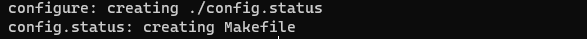
\includegraphics[width=0.9\textwidth]{images/4.png}
    \caption{Result of succeeded configuration}
\end{figure}

\subsection{Build}
After you surely prepared source codes are intact, checked configuration was successful, run this command:\\

\texttt{make -j <cpu-core-count>}\\

You can run \texttt{make} without \texttt{-j} switch, then your compilation process will slow down, because 
such switch enables parallrel compilation with specified amount of cores.

This process takes long time, depends on performance of processor. On my machine, it took 30 minutes 
with \textbf{Intel i7-10875H} with 8 cores. If C++ omitted from configuration, build time can be drastically reduced.

\begin{figure}[!htbp]
    \centering
    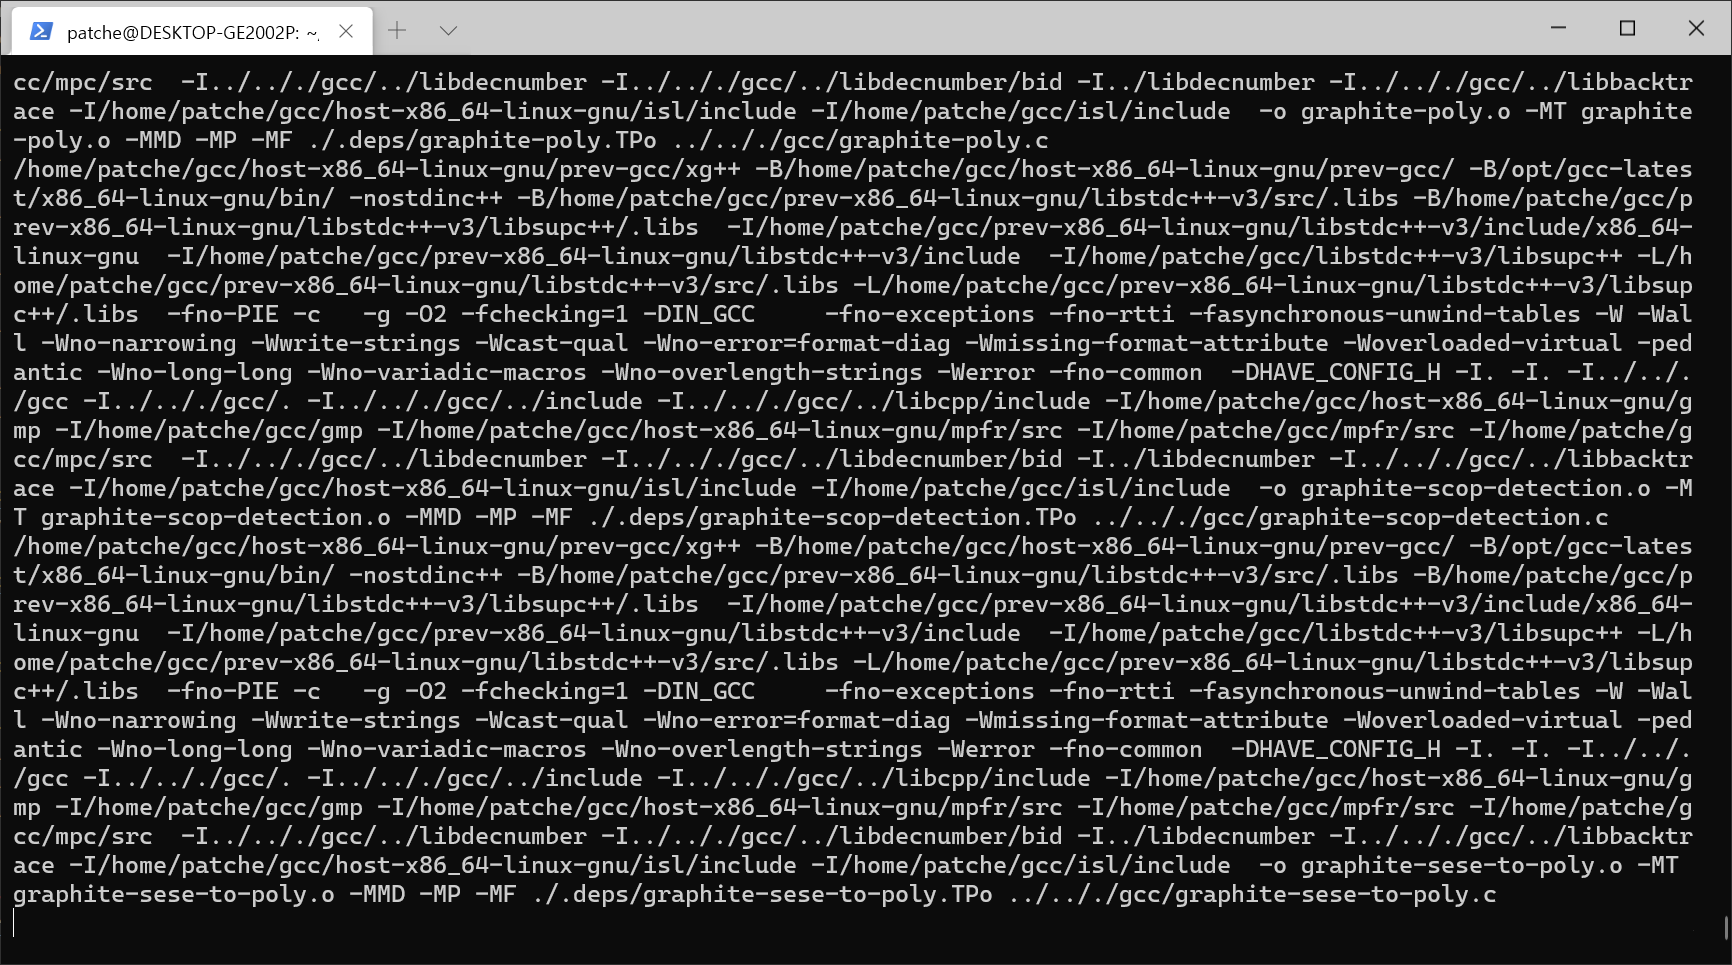
\includegraphics[width=0.8\textwidth]{images/6.png}
    \caption{GCC building proceess via GNU Make}
\end{figure}

\begin{figure}[!htbp]
    \centering
    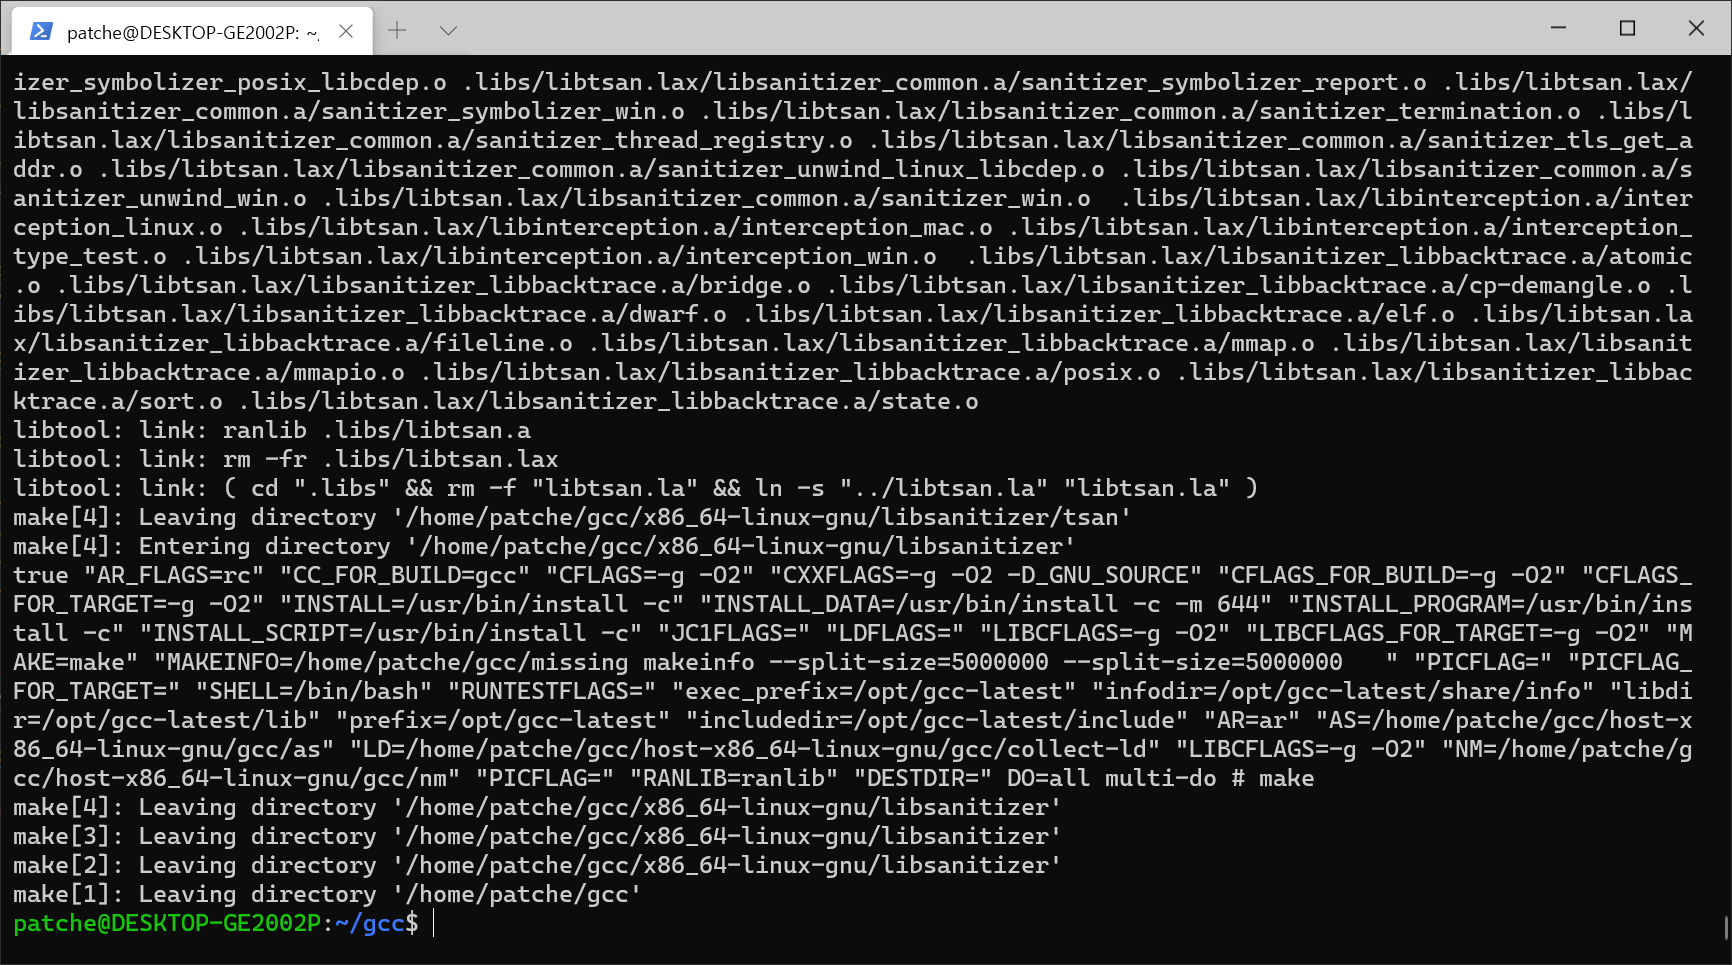
\includegraphics[width=0.8\textwidth]{images/7.png}
    \caption{GNU Make terminated with success}
\end{figure}


\subsection{Install}

Once \texttt{make} is finished, run command \texttt{make install}. If you are trying
this command with gcc configured \texttt{prefix} to privileged directory, make sure
you have enough permission or in superuser.

\begin{figure}[!htbp]
    \centering
    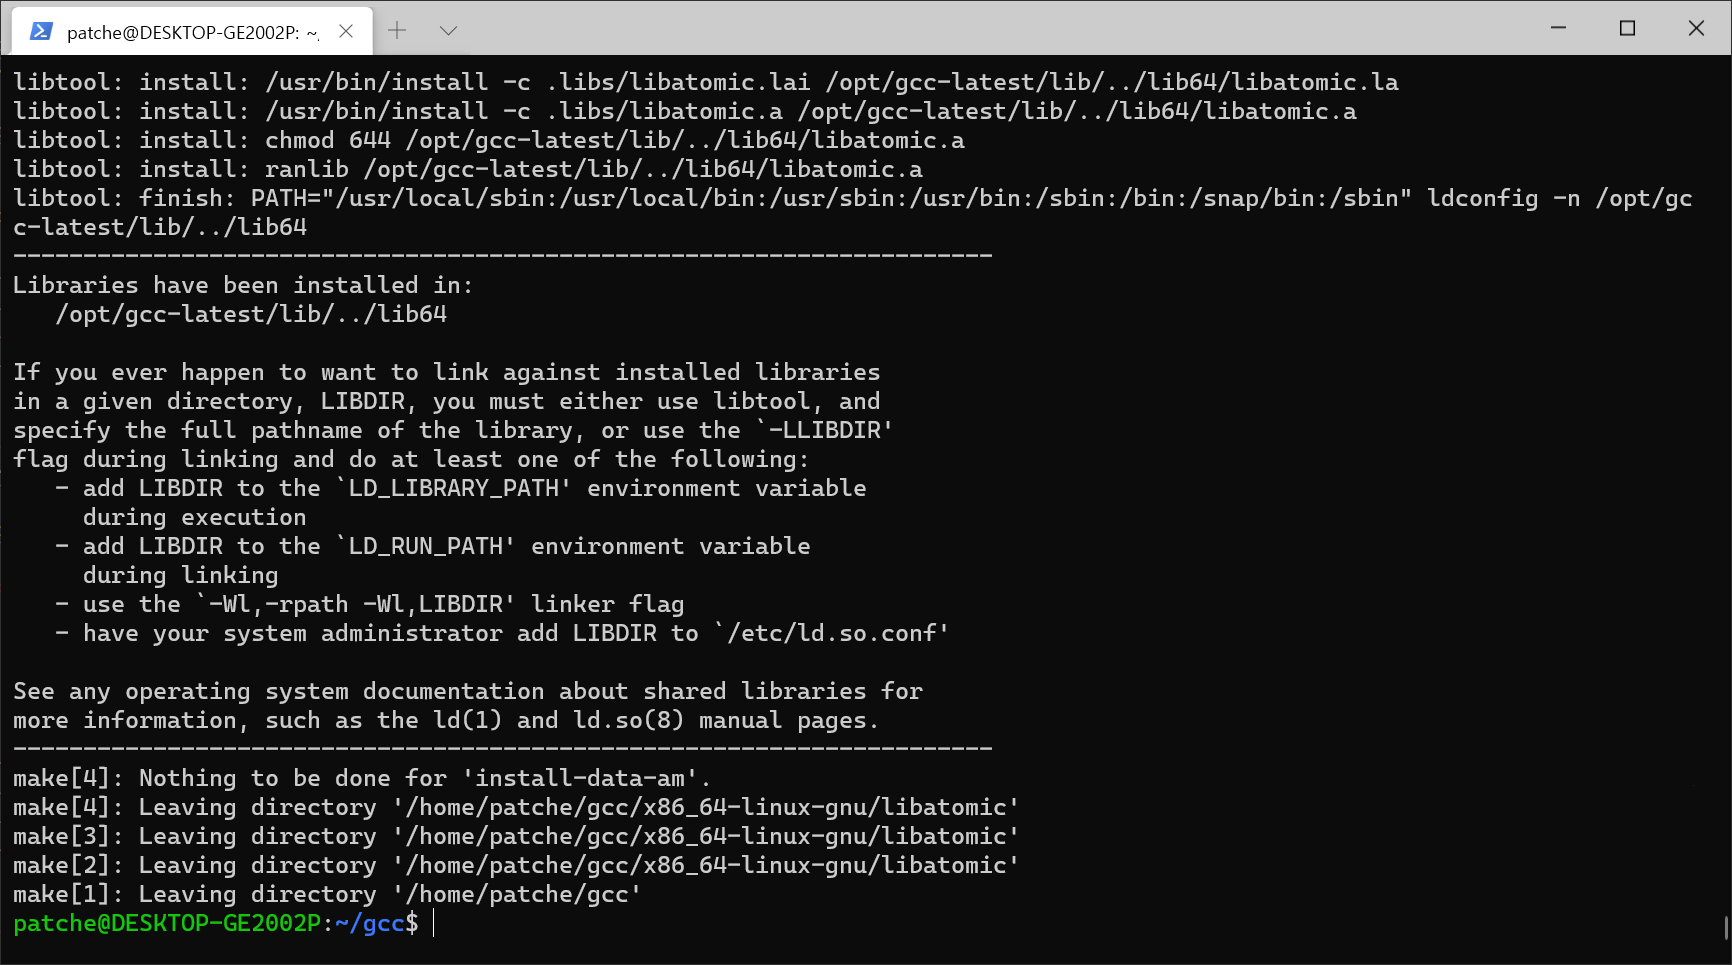
\includegraphics[width=0.8\textwidth]{images/8.png}
    \caption{After \texttt{make install}}
\end{figure}

Now check directory that you designated as \texttt{prefix}, you can see installed gcc
files in good shape. Executable gcc binaries are in \texttt{bin} folder.

\begin{figure}[!htbp]
    \centering
    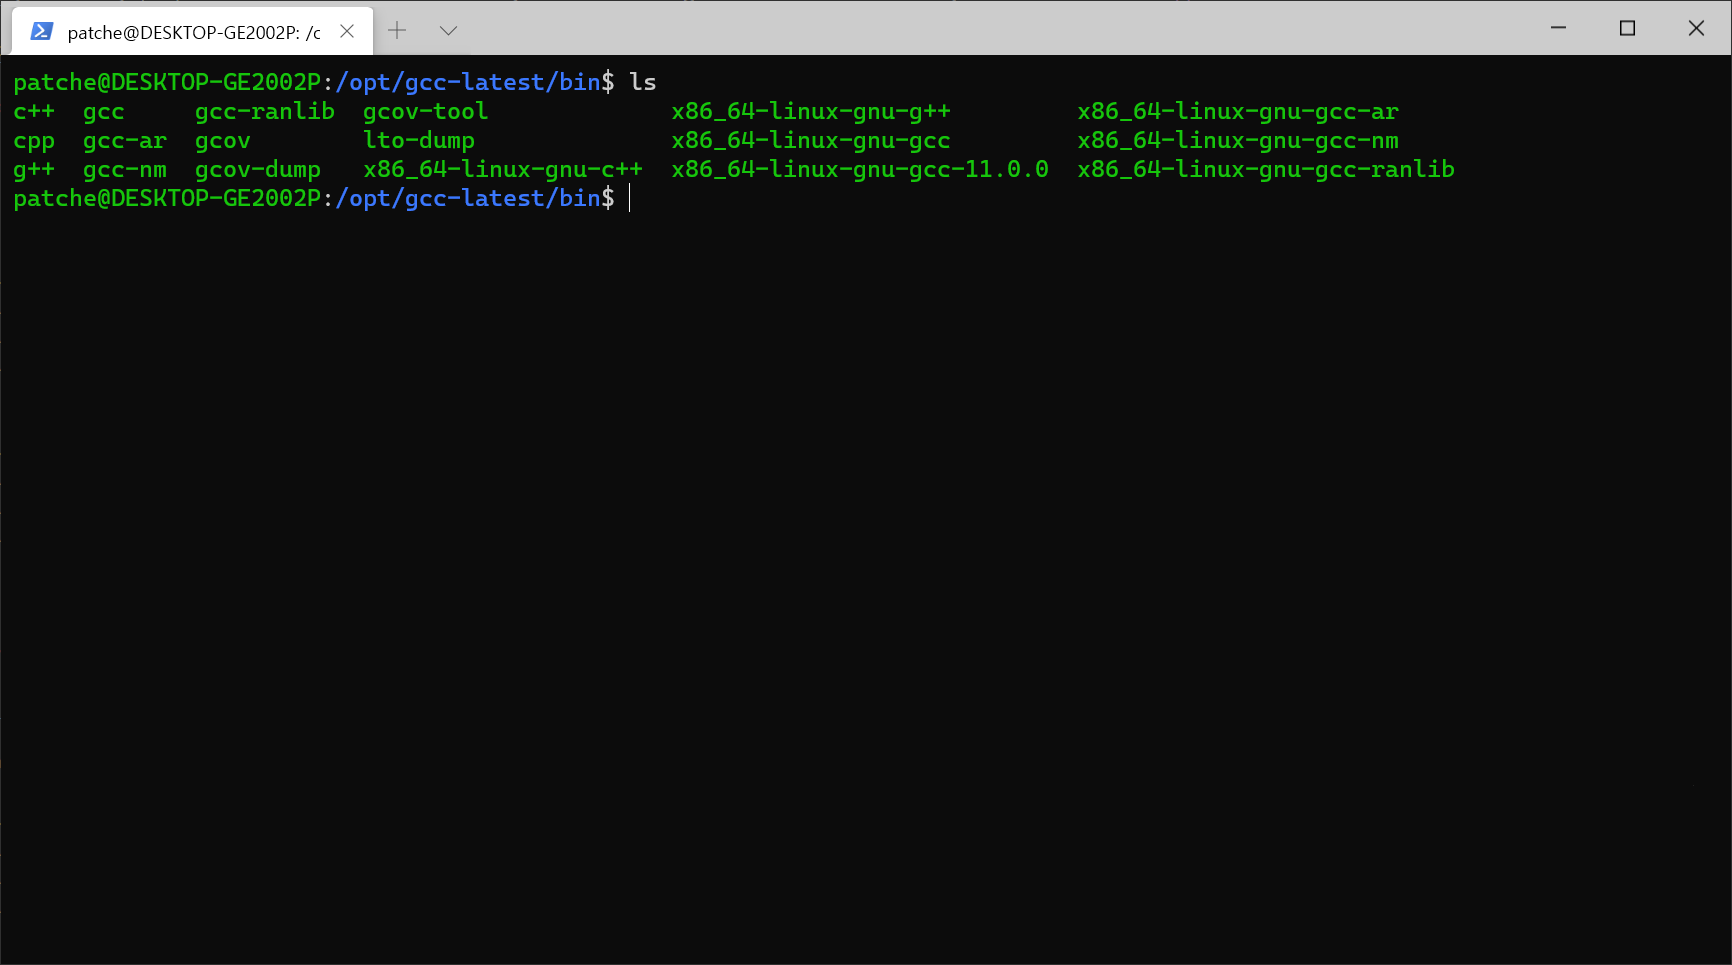
\includegraphics[width=0.8\textwidth]{images/9.png}
    \caption{After \texttt{Executable GCC binaries}}
\end{figure}

These binaries can be executed with relative/absolute path, however, we don't use
compilers in such way, but like `ls` or `chmod' things. To make this possible, add the \texttt{bin}
folder to \texttt{PATH} environemnt variable.

\begin{figure}[!htbp]
    \centering
    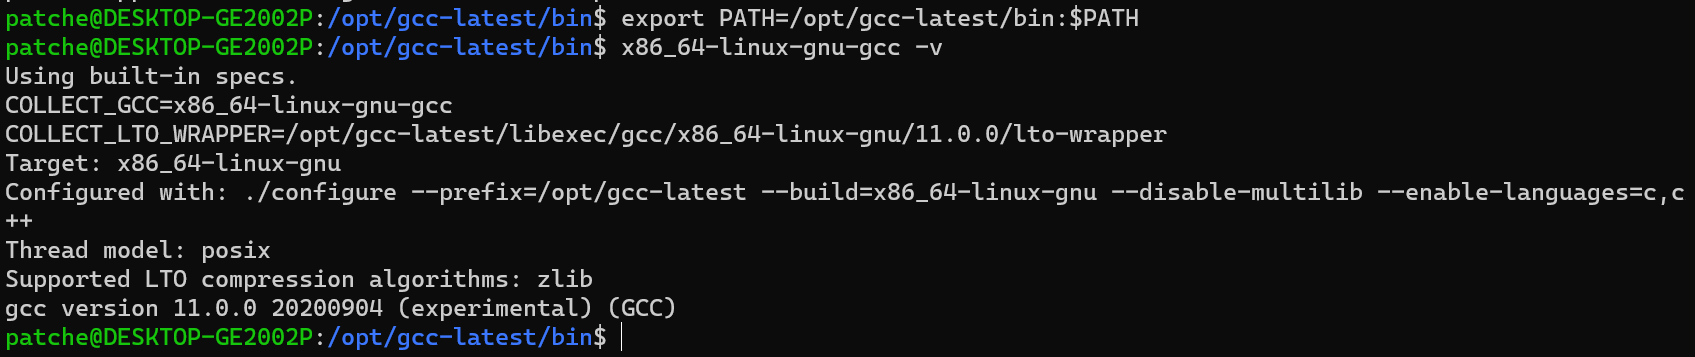
\includegraphics[width=0.8\textwidth]{images/10.png}
    \caption{\texttt{PATH} setup}
\end{figure}

\section{Conclusion}

Doing this assignment, I reviewed about how linux programs are distributed and installed.
Although package managers provide users pre-built packages with typical option for each architectures,
some of unique packages are not supported correctly, Manual compilation is required in such case. 
Therefore, It is important that keeping such knowledge in mind, to utilize linux more stable.

\section*{APPENDIX}

To prove the works above are conducted by myself, Attach this screenshot:

\begin{figure}[!htbp]
    \centering
    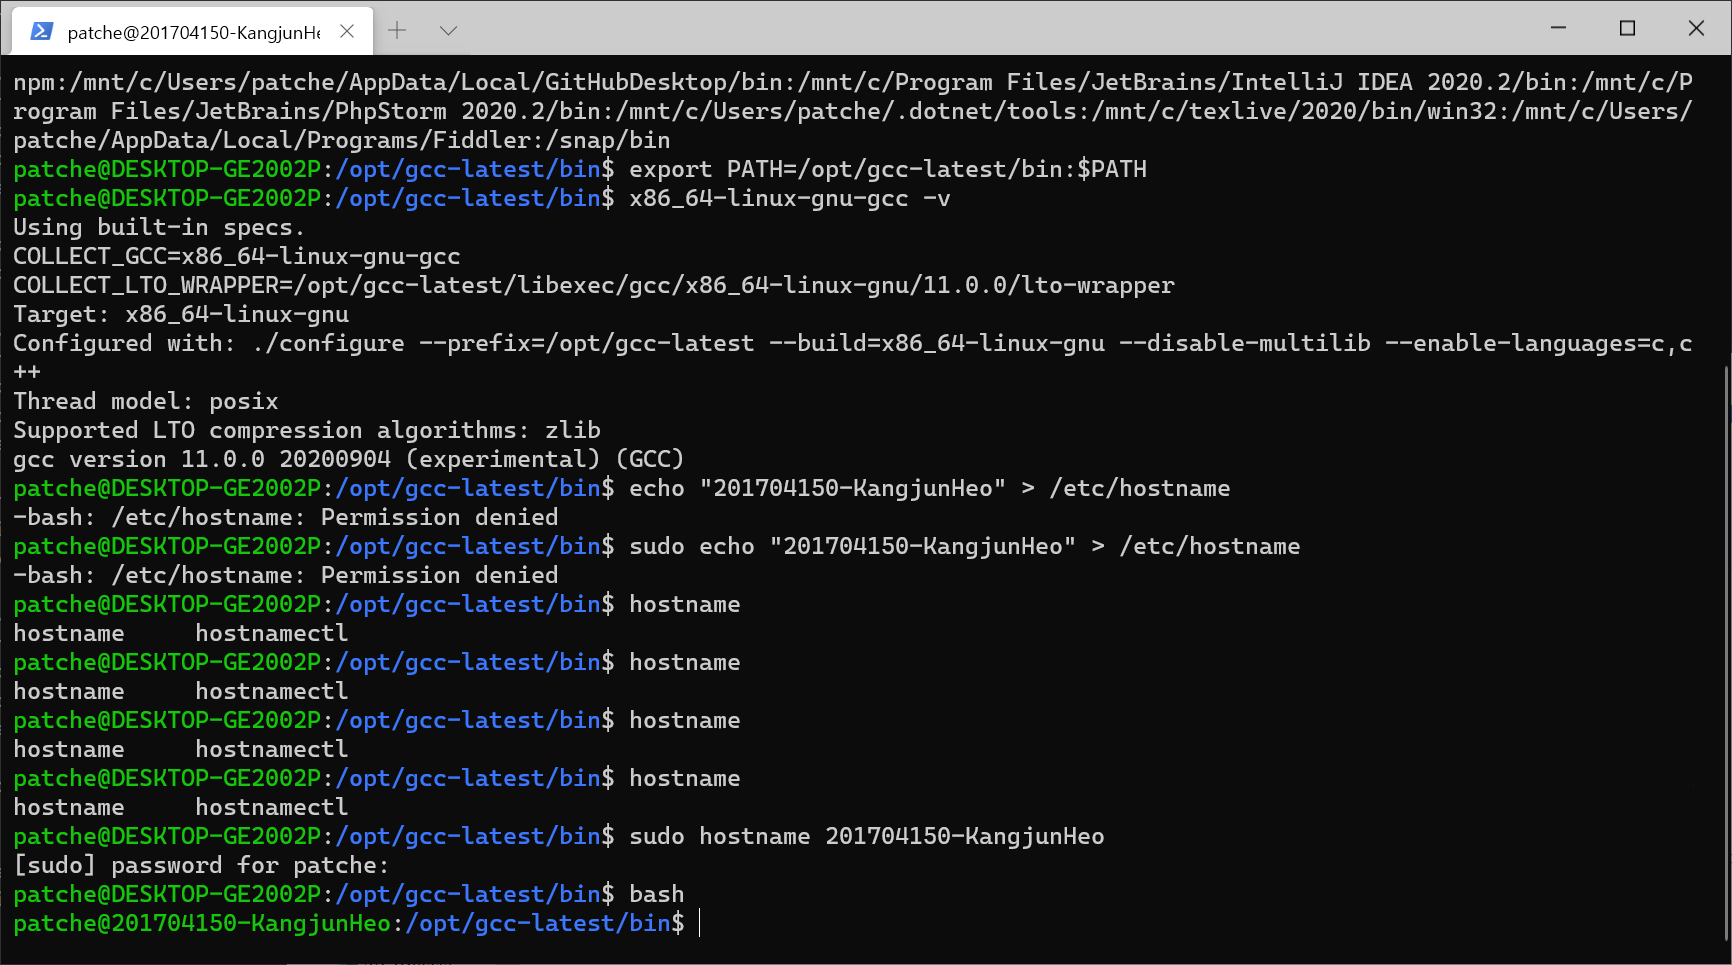
\includegraphics[width=0.8\textwidth]{images/11.png}
\end{figure}


\section*{REFERENCES}

\begin{itemize}
    \item GNU GCC Install Manual: https://gcc.gnu.org/install/
    \item GNU Make: https://www.gnu.org/software/make/
    \item Configure option: https://github.com/docker-library/gcc
\end{itemize}

\end{document}